\documentclass[twocolumn, amsmath, amsfonts, amssymb, trackchanges]{aastex62}
\usepackage{mathtools}
\usepackage{natbib}
\usepackage{bm}
\newcommand{\vdag}{(v)^\dagger}
\newcommand\aastex{AAS\TeX}
\newcommand\latex{La\TeX}


\newcommand{\Div}[1]{\ensuremath{\nabla\cdot\left( #1\right)}}
\newcommand{\DivU}{\ensuremath{\nabla\cdot\bm{u}}}
\newcommand{\angles}[1]{\ensuremath{\left\langle #1 \right\rangle}}
\newcommand{\td}[1]{\ensuremath{\widetilde{#1}}}
\newcommand{\KSstat}[1]{\ensuremath{\overline{\text{KS}(#1)}}}
\newcommand{\grad}{\ensuremath{\nabla}}
\newcommand{\RB}{Rayleigh-B\'{e}nard }
\newcommand{\stressT}{\ensuremath{\bm{\bar{\bar{\Pi}}}}}
\newcommand{\lilstressT}{\ensuremath{\bm{\bar{\bar{\sigma}}}}}
\newcommand{\nrho}{\ensuremath{n_{\rho}}}
\newcommand{\approptoinn}[2]{\mathrel{\vcenter{
	\offinterlineskip\halign{\hfil$##$\cr
	#1\propto\cr\noalign{\kern2pt}#1\sim\cr\noalign{\kern-2pt}}}}}

\newcommand{\appropto}{\mathpalette\approptoinn\relax}
\newcommand{\pro}{\ensuremath{\text{Ro}_{\text{p}}}}
\newcommand{\con}{\ensuremath{\text{Ro}_{\text{c}}}}

\usepackage{color}
\newcommand{\gv}[1]{{\color{blue} #1}}

%% Tells LaTeX to search for image files in the 
%% current directory as well as in the figures/ folder.
\graphicspath{{./}{figs/}{../tex/figs/}}


\received{\today}
\revised{\today}
\accepted{??}%\today}
\submitjournal{ApJ}

%%%%%%%%%%%%%%%%%%%%%%%%%%%%%%%%%%%%%%%%%%%%%%%%%%%%%%%%%%%%%%%%%%%%%%%%%%%%%%%
%% TITLE & AUTHORS
\shorttitle{Stratified Thermals}
\shortauthors{Anders et al.}

\begin{document}
\title{Entrainment of low Mach number thermals in stratified domains}

\correspondingauthor{Evan H. Anders}
\email{evan.anders@colorado.edu}

\author[0000-0002-3433-4733]{Evan H. Anders}
\affil{Dept. Astrophysical \& Planetary Sciences, University of Colorado -- Boulder, Boulder, CO 80309, USA}
\affil{Laboratory for Atmospheric and Space Physics, Boulder, CO 80303, USA}
\author[0000-0002-7635-9728]{Daniel Lecoanet}
\affil{Stuff}
\author[0000-0001-8935-219X]{Benjamin P. Brown}
\affil{Dept. Astrophysical \& Planetary Sciences, University of Colorado -- Boulder, Boulder, CO 80309, USA}
\affil{Laboratory for Atmospheric and Space Physics, Boulder, CO 80303, USA}


\begin{abstract}
\end{abstract}

\keywords{hydrodynamics --- turbulence --- entrainment}

%%%%% Body of the paper
%%%%%%%%%%%%%%%%%%%%%%%%%%%%%%%%%%%%%%%%%%%%%%%%%%%%%%%%%%%%%%%%%%%%%
%% INTRODUCTION
\section{Introduction}
\label{sec:intro}
Recent observations of solar convection have revealed a convective conundrum.
Power spectra have revealed weaker flows than anticipated at large length scales,
calling into question the existence of so-called ``giant cells'' driven by deep
convection which would manifest as powerful, large-scale motions at the solar
surface. This discrepancy between theory and observations has called into question
our fundamental understanding of convection, sparking fruitful investigations into
the nature of convection in the Sun.

\cite{spruit1997} hypothesized that convective motions may be driven entirely by
cool downflows at the surface of the Sun, and \citet{brandenburg2016} expanded
upon this ``entropy rain'' hypothesis. Brandenburg's work includes a careful
expansion of mixing length theory to incorporate flux contributions from nonlocal
convective motions, and handles this theory in a horizontally-averaged sense.
He includes some discussion of possible flow morphologies which could be manifestations
of this entropy rain, and even includes some brief simulations of propogating
Hill vortices. However, these simulations and discussions did not include 
include a fundamental piece of entropy rain: it is buoyant, and has an entropy
deviation from the background atmosphere.

If entropy rain does evolve into downward propagating buoyant vortex rings, it is
important to understand how buoyancy effects the filling factor of these basic
convective elements. In the context of Earth's atmosphere, so-called ``thermals''
are thought to be the nucleus of cloud formation. Thermals are buoyant areas
of fluid which evolve into propagating buoyant vortex rings, and their
evolution in the Boussinesq limit have been well studied in the laboratory
for decades (see e.g., CITE), and more recently have been studied through
Direct Numerical Simulation (DNS) in the laminar and turbulent regime
\citep{lecoanet&jeevanjee2018}. One fundamental result of these studies of
thermals is that they experience a large degree of entrainment: their size expands
with height and their propagation velocity slows despite their buoyant nature.
However, we do not know of a study in which the propagation of these thermals,
and thus the nature of their entrainment, is affected by a 
significant atmospheric stratification.

In the absence of buoyantly-induced entrainment, \citet{brandenburg2016}
suggests that the filling factor, $f$, of vortex rings should decrease like
$f \propto \rho^{\alpha}$ for horizontal compression and $f \propto \rho^{\alpha}$ for 
spherical compression. On the other hand, the filling factor of Boussinesq
thermals \emph{increases} like $f \propto d$, where $d$ is the depth propagated.
In this work, we extend the study of \citet{lecoanet&jeevanjee2018} to study
the propagation of low-Mach number, cold thermals in stratified domains, and how
buoyant entrainment affects the scaling of their filling factor with depth. If
buoyant entrainment is a dominant effect, it is possible that these buoyant vortex rings
would simply grow too large and stall before reaching the bottom of the solar convection zone.
On the other hand, if the compression effects suggested by \citet{brandenburg2016} are the
dominant effect, then it is possible that these thermals could propagate to the bottom of the solar
convection zone, or potentially shrink to a sufficiently small size where thermal dissipation is
significant.

We lay out our work as follows. In section \ref{sec:theory}, we develop a theoretical description
of thermals in a stratified domain. In section \ref{sec:experiment}, we describe and verify
the experiments conducted in this work. In section \ref{sec:results}, we compare the results
of our experiments to the theory developed in section \ref{sec:theory}. Finally, in section
\ref{sec:discussion}, we discuss what our results imply for the entropy rain hypothesis.

%%%%%%%%%%%%%%%%%%%%%%%%%%%%%%%%%%%%%%%%%%%%%%%%%%%%%%%%%%%%%%%%%%%%%%%%%%%%%%
%% THEORY SECTION
\section{Theory}
\label{sec:theory}

\subsection{Phenomenological description of thermal evolution}
We show pictorally the evolution of a cold thermal from rest in 
Fig.~\ref{fig:evolution_colormeshes}. In Fig.~\ref{fig:evolution_colormeshes}a,
the evolution of a thermal in a weakly stratified domain with
$n_\rho = 0.5$ density scale heights is shown. In Fig.~\ref{fig:evolution_colormeshes}b,
the evolution of a thermal in an appreciably stratified domain with
$n_\rho = 3$ density scale heights is shown. While the initial conditions are
identical in both domains (spherical specific entropy perturbations of the
same magnitude whose diameters are 5\% of the domain depth), and while in both cases
the thermal quickly evolves into a propagating buoyant vortex ring, we find that the
$n_\rho = 0.5$ case entrains and grows with depth, similarly to the Boussinesq regime.
On the other hand, the $n_\rho = 3$ case has a radius which remains approximately constant
over time, and it reaches the bottom of the domain in many fewer nondimensional freefall
time units.

\begin{figure*}[t!]
    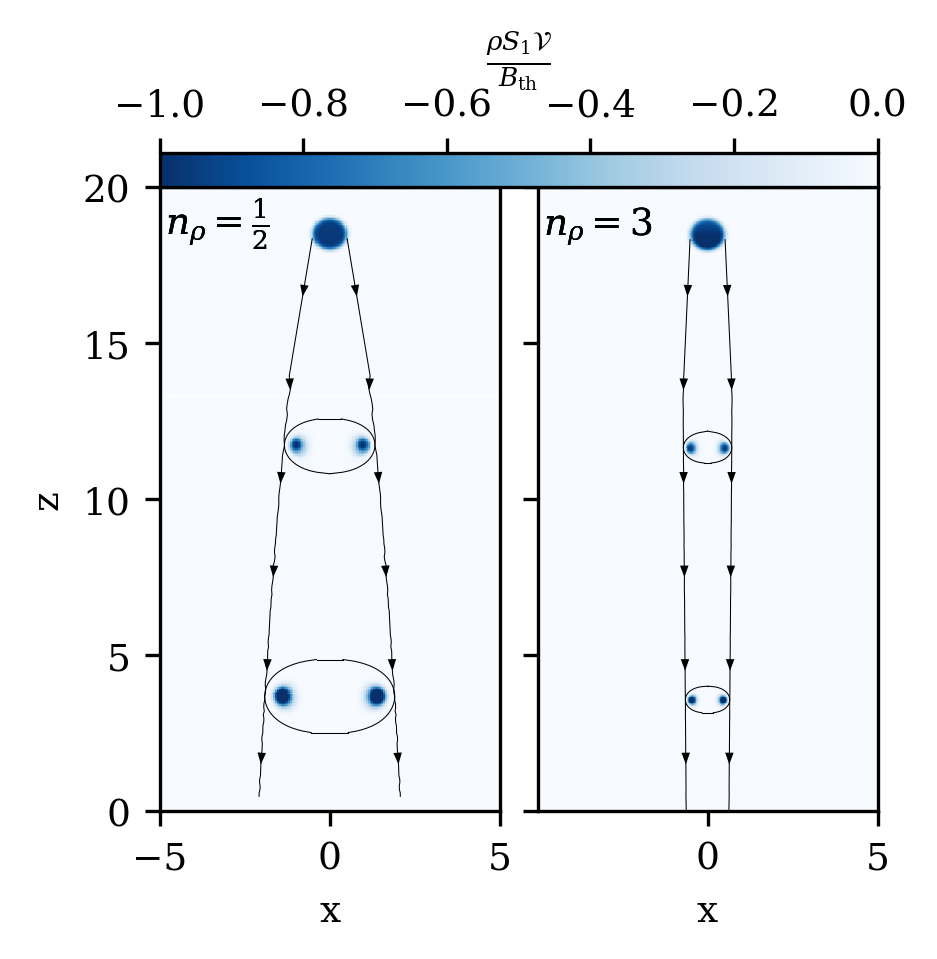
\includegraphics[width=\columnwidth]{evolution_colormeshes.png}
    \caption{
    \label{fig:evolution_colormeshes} }
\end{figure*}


\subsection{Theoretical description of thermal evolution}
The evolution of thermals as buoyant vortex rings has been well described in
the unstratified, Boussinesq limit for decades (as early as e.g., CITE, and
see \citet{lecoanet&jeevanjee2018} for other sources). Buoyant motions 
in the atmospheres of stars and planets are generally large enough to feel the
atmospheric stratification, and therefore a more thorough tratment of the
evolution of thermals in stratified domains is required to understand the nature
of thermal entrainment in nature.

In this work, we focus on the non-dissipative, low Mach number regime, 
in which the ideal anelastic equations are a decent approximation to the fully
compressible equations. In this regime, the buoyancy is directly proportional to the
specific entropy. In the absence of diffusion, or in the limit where diffusivities
are sufficiently small, the volume-integrated total entropy is constant,
\begin{equation}
B \equiv \int_{\mathcal{V}} \rho\, s\, dV = \text{const},
\end{equation}
where $s = c_V \ln T - R \ln\rho$ is the specific entropy, with $c_V$ the
specific heat at constant volume and $R$ the ideal gas constant.

In a stratified domain, the hydrodynamic impulse is defined
\citet{shivamoggi2010},
\begin{equation}
\bm{I} = \frac{1}{2}\int_{\mathcal{V}} \bm{x}\times(\grad\times(\rho\bm{u}))dV,
\end{equation}
where $\bm{x}$ is the position vector, $\bm{u}$ is vector velocity, $\rho$ is density,
and $\mathcal{V}$ is the volume being integrated over. Furthermore, changes in the impulse
can be expressed
\begin{equation}
\frac{\partial\bm{I}}{\partial t} = \int_{\mathcal{V}}\frac{\partial}{\partial t}(\rho \bm{u})dV
= B\hat{z} + S,
\end{equation}
where $S$ is a combination of surface terms that disappears upon appropriate boundary conditions
on $\mathcal{V}$ \citep{shivamoggi2010}. As we have assumed that the buoyancy, $B$, is constant,
we can straightforwardly integrate
\begin{equation}
I_z = B t + I_0,
\end{equation}
for some constant $I_0$.

(need to work through this section carefully).
Assuming an adiabatically stratified atmosphere in
hydrostatic equilibrium, the vertical momentum equation is
\begin{equation}
 = - \partial_z \varpi +  g\frac{S_1}{c_P},
\label{eqn:buoyancy}
\end{equation}
where $w$ is vertical velocity, $S_1$ is specific entropy, $\varpi$ is the reduced pressure,
$D/Dt = \partial_t + (\bm{u}\cdot\grad)$ is the (eulerian? lagrangian?)
derivative, $g$ is gravity, and $c_P$ is the specific heat at constant pressure.
In the anelastic approximation, the density stratification is constant in time. 
OH GOD I DON'T KNOW THIS MATH WELL MAGIC MAGIC MAGIC.
By doing magic, we arrive at
\begin{equation}
P_z = \beta B t + P_0.
\end{equation}

Under the assumption that the thermal develops into a thin-core 
propagating vortex ring whose vortex core is radius $r$ away from the axis of symmetry, 
the impulse can be approximated as $I_z \approx \pi \rho r^2 \Gamma$, where 
$\Gamma$ is the circulation of the thermal vortex, which we assume to be constant. 
Rearranging, we find our first result,
\begin{equation}
r = \sqrt{\frac{B t + I_0}{\pi\rho\Gamma}}.
\label{eqn:r_theory}
\end{equation}
In the limit where $\rho \rightarrow \text{constant}$, as in the Boussinesq regime,
we retrieve the $r \propto \sqrt{t}$ scaling found in the Boussinesq regime by
\citet{lecoanet&jeevanjee2018}. We find that the inclusion of stratification adds the
additional complexity of $r \propto \rho^{-1/2}$, such that downward-propogating 
vortex rings (as studied here) will not entrain to the same degree as boussinesq thermals,
and upward-propogating rings will entrain more.

We further assume that the volume-integrated momentum, $P_z \approx \rho V w_{th}$,
where $w_{th}$ is the vertical velocity of the thermal as a whole, and the volume
of the fluid region propogating with the thermal is a spheroid, $V = V_0 r^3$, for
some constant $V_0$. Plugging Eqn.~\ref{eqn:r_theory} into this approximation, we
find that
\begin{equation}
\rho^{-1/2}w = \left(\frac{(\pi\Gamma)^{3/2}}{V_0}\right)\frac{\beta B t + M_0}{(B t + I_0)^{3/2}}.
\end{equation}
Substituting $w = dz/dt$ and $\tau \equiv (Bt + I_0)/\Gamma$, We retrieve
\begin{equation}
\frac{dz}{\sqrt{\rho(z)}} 
= \left(\frac{\pi^{3/2}\Gamma}{V_0}\right)
\left(\beta\Gamma\tau^{-1/2} + [M_0 - \beta I_0]\tau^{-3/2}\right)d\tau.
\label{eqn:general_theory}
\end{equation}
If the atmospheric stratification in which the thermal is falling is known, this
result can be straightforwardly integrated with $\rho(z)$ plugged in in order to
find the position of the thermal versus time. While we will leave this result
general for now, we will plug in our polytropic stratification at the end of
section \ref{sec:experiment}, and show that the resulting expression does a
good job of explaining the evolution of thermals in these atmospheres in
section \ref{sec:results}.

%%%%%%%%%%%%%%%%%%%%%%%%%%%%%%%%%%%%%%%%%%%%%%%%%%%%%%%%%%%%%%%%%%%%%%%%%%%%%%%
%% EXPERIMENT SECTION
\section{Experiment} 
\label{sec:experiment}


\subsection{Anelastic Simulations}
In this work, we primarily study the evolution of 2D, azimuthally symmetric, anelastic
thermals in cylindrical coordinates. 
We later verify that these simulations produce the same results a 3D fully compressible
simulations in 3D cartesian domains (see sec. REF). 
The LBR anelastic equations are \citep{lecoanet&all2014},
\begin{gather}
\td{\grad}\cdot\td{\bm{u}} = -\td{w}\partial_{\tilde{z}} \ln\rho_0 \\
\frac{D \td{\bm{u}}}{D \td{t}} = -\td{\grad} \td{\varpi} + g\frac{\td{S_1}}{c_P}\hat{z} + \frac{1}{\rho_0}\td{\grad}\cdot\left(\mu\td{\lilstressT}\right) \\
\frac{D \td{S_1}}{D\td{t}} = \frac{1}{\rho c_P}\td{\grad}\cdot\left(\kappa T_0 \td{\grad} \td{S_1}\right) + \frac{\mu}{\rho_0 T_0}\td{\sigma_{ij}}\partial_{\td{x_i}}\td{u_j}.
\end{gather}
where terms with tildes are dimensional, and where
$D/D\td{t} = \partial/\partial \td{t} + \td{\bm{u}}\cdot\td{\grad}$. In our azimuthally symetric
domain, we assume that $\partial_\phi = 0$; as the initial conditions of our simulations are at rest and have
no azimuthal velocity, $u_\phi$, we assume that $u_\phi = 0$; therefore $\bm{u} = u_r \hat{r} + w\hat{z}$. 
Under this approximation, the components of the stress tensor are
\begin{equation}
\begin{split}
&\td{\sigma}_{rr} = 2\frac{\partial \td{u_r}}{\partial \td{r}} - \frac{2}{3}\td{\grad}\cdot\td{\bm{u}},\,\,\,\,\,\,
\td{\sigma}_{rz}     = \td{\sigma}_{zr} = \frac{\partial \td{w}}{\partial \td{r}} + \frac{\partial \td{u_r}}{\partial \td{z}}, \\
&\td{\sigma}_{\phi\phi} = 2\frac{\td{u_r}}{\td{r}} - \frac{2}{3}\td{\grad}\cdot\td{\bm{u}},\,\,\,\,\,\,\,
\td{\sigma}_{r\phi}  = \td{\sigma}_{\phi r}  = 0, \\
&\td{\sigma}_{zz}       = 2\frac{\partial \td{w}}{\partial \td{z}} - \frac{2}{3}\td{\grad}\cdot\td{\bm{u}}, \,\,\,\,\,\,
\td{\sigma}_{\phi z} = \td{\sigma}_{z \phi}  = 0,\qquad
\end{split}
\end{equation}
Furthermore, we assume that the dynamic viscosity, $\mu = \rho \nu$, and the
thermal conductivity, $\kappa = \rho \chi$, are both uniform throughout the domain.
The diffusivities
$\nu$ and $\chi$ therefore scale inversely with the density.

We nondimensionalize these equations in the same manner as in
\citet{lecoanet&jeevanjee2018} such that
the length scale is the diameter of the initial thermal perturbation
and the velocity scale is the freefall velocity. The timescale is thus
the freefall crossing time of this unit length. Mathematically,
\begin{equation}
\begin{split}
\td{\grad}\rightarrow(\td{L}_{th}^{-1})\grad, \qquad&
\td{S}_1 \rightarrow(\Delta\td{S})S_1,\\
\td{\bm{u}} \rightarrow (\td{u}_{th})\bm{u}, \qquad&
\td{\varpi} \rightarrow (\td{u}_{th}^2)\varpi,\\
\partial_{\tilde{t}} \rightarrow (\td{u}_{th}/\td{L}_{th})\partial_t,\qquad&
\end{split}
\end{equation}
with
\begin{equation}
\tilde{u}_{th}^2 = \frac{g \tilde{L}_{th} \Delta \tilde{s}}{c_P}, \qquad
\text{Re}_{\text{ff}} = \frac{\tilde{u}_{th} \tilde{L}_{th}}{\nu}, \qquad
\text{Pr}_{\text{ff}} = \frac{\tilde{u}_{th} \tilde{L}_{th}}{\chi}.
\end{equation}
As the diffusivities scale with depth, Re$_{\text{ff}}$ is specified at the
thermal's initial depth.
The resulting equations are,
\begin{gather}
\DivU = -w \partial_z \ln\rho_0, \\
\begin{split}
\partial_t \bm{u} + \bm{u}\cdot\grad\bm{u} =& \\
- \grad \varpi + S_1\hat{z} &
+ \frac{1}{\text{Re}_{\text{ff}}}\left[\grad^2 \bm{u} + \frac{1}{3}\grad(\DivU)\right] 
\end{split}\\
\begin{split}
\partial_t S_1 + \bm{u}\cdot\grad S_1 =& \\
\frac{1}{\text{Re}_{\text{ff}}}\left(\frac{1}{\text{Pr}_{\text{ff}}\rho_0c_P }\right.&[\grad^2 S_1 + \partial_z\ln T_0 \cdot\partial_z S_1]\\
&+ \left.\frac{-(\grad_{ad})}{\rho_0 T_0}\sigma_{ij}\partial_{x_i}u_j \right)
\end{split}
\end{gather}
where in this nondimensionalization, the adiabatic temperature gradient is defined
in the next subsection.

\subsection{Atmosphere \& Initial conditions}
We study an ideal gas whose equation of state is $P = \rho T$ and whose stratification
is a perfectly adiabatic polytrope,
\begin{gather}
T_0 = 1 + (\grad_{\text{ad}})(z - L_z) \\
\rho_0 = T_0^{m_{\text{ad}}},
\end{gather}
where $m_{\text{ad}} = (\gamma-1)^{-1}$, and the adiabatic temperature 
gradient in these nondimensional atmospheres is
$$
\grad_{\text{ad}} = -\frac{(e^{n_\rho/m_{ad}} - 1)}{L_z}\frac{m_{ad} + 1}{c_P},
$$
where $L_z$ is the atmospheric depth in units of thermal diameters.
 
To initialize the simulation, we specify a spherical initial specific entropy perturbation,
\begin{equation}
S_1 = - A(1 - \text{erf}\left(\frac{r' - r_{th}}{\delta}\right))/2,
\label{eqn:thermal_IC}
\end{equation}
where $A = 1$ for our scaled equations.
Here, $r' = \sqrt{r^2 + (z - z_0)^2}$, where $z_0 = L_z - 3*r_{th}$,
with the thermal radius set as $r_{th} = 0.5$, and a smoothing width, $\delta = 0.1$.



\subsection{Fully Compressible Simulations}
In order to verify the validity of our 2D Anelastic simulations, we evolve select
thermals according to the 3D Navier Stokes equations in a cartesian domain. We use
the $(T, \ln\rho)$ formulation of the equations in which we have previously studied fully compressible
convection at low and high Mach number \citep{anders&brown2017, lecoanet&all2014},
\begin{gather}
\frac{D \ln\rho}{Dt} + \DivU = 0 \\
\frac{D \bm{u}}{D t} = -\grad T - T\grad\ln\rho - g\hat{z} + \frac{1}{\rho}\grad\cdot\left(\mu\lilstressT\right) \\
\frac{D T}{Dt} + (\gamma-1)T\DivU  = \frac{1}{\rho c_V}\grad\cdot\left(\kappa \grad T\right) + \frac{\mu}{\rho c_V}\sigma_{ij}\partial_{x_i}u_j.
\end{gather}
where the viscous stress tensor is defined as
\begin{equation}
\sigma_{ij} = \left(\partial_{x_i}u_j + \partial_{x_j}u_i - \frac{2}{3}\delta_{ij}\grad\cdot\bm{u}\right).
\end{equation}
These equations are nondimensionalized on the temperature gradient length scale such that
$\grad_{\text{ad}} = -1$ and the nondimensional timescale is the sound crossing time of that
unit length.  

In setting the specific entropy, $S = c_V \ln T - R^{-1}\ln\rho$, to an equivalent condition
to that specified in  Eqn.~\ref{eqn:thermal_IC}, we note that it is essential that the
initial perturbation be in pressure equilibrium. The set of initial conditions that achieves this
is
\begin{equation}
\ln\rho_1 = S_1/c_P, \qquad T_1 = T_0(e^{-\ln\rho_1} - 1).
\end{equation}
We specify the magnitude of the initial entropy perturbations as 
$A = \epsilon = 10^{-4}$, such that the mach number of the resultant thermal is O($10^{-2}$) or less.

The depth of the atmosphere in these fully compressible domains is set by the number of density
scale heights as $L_z = e^{n_\rho/m_{ad}} - 1$, and in order to compare results from these
simulations to our nondimensionalized thermal simulations, we rescale all length scales in
post-processing by $\ell = 20/L_z$, all timescales by $\tau = \sqrt{\ell \epsilon}$, and
the entropy by $s = \epsilon^{-1}$.


\subsection{Solution for thermal evolution in a Polytrope}
Here we take the general theory described in Eqn.~\ref{eqn:general_theory} and apply it
to the specific case of the polytropes we study here. 
We note that, $\rho_0 = T_0^{m_{ad}}$ and
$dT_0 = (\grad_{\text{ad}}) dz$, such that we must solve
\begin{equation}
T_0^{-m_{ad}/2} dT_0 
= \left(\frac{\pi^{3/2}\Gamma\grad_{\text{ad}}}{V_0}\right)
\left(\beta\Gamma\tau^{-1/2} + [M_0 - \beta I_0]\tau^{-3/2}\right)d\tau.
\label{eqn:general_theory}
\end{equation}
Assuming that $m_{ad} < 2$ and through the use of simple power law integrals, we
find that
\begin{equation}
T_0(t) = \left(C[\xi(\tau) - \xi(\tau_0)] + T_0(t_0)^{1/\alpha}  \right)^{\alpha},
\end{equation}
with
\begin{equation}
\xi(\tau) = \beta\Gamma\tau^{1/2} - (M_0 - \beta I_0) \tau^{-1/2},
\end{equation}
$C \equiv (2 \pi^{3/2} \Gamma (\grad_{\text{ad}}))/(\alpha V_0 B)$



\subsection{Verification of 2D Anelastic approximation}
blah blah blah comparison of 2D and 3D blah blah blah. z v t, r v z, w v z. Also side-by-side
pictoral comparison with diff. 

%%%%%%%%%%%%%%%%%%%%%%%%%%%%%%%%%%%%%%%%%%%%%%%%%%%%%%%%%%%%%%%%%%%%%%%%%%%%%%%
%% RESULTS SECTION
\section{Results}
\label{sec:results}
Picture of a big old grid of z v t, r v z, w v z.

Pretty picture showing thermal evolution (comparing low and high stratification).

Verification of theory by simulations

Table of found parameters for the fits

Two regimes: stalling and falling.


%%%%%%%%%%%%%%%%%%%%%%%%%%%%%%%%%%%%%%%%%%%%%%%%%%%%%%%%%%%%%%%%%%%%%%%%%%%%%%%
%% CONCLUSION SECTION
\section{Discussion}
\label{sec:discussion}
Wild speculation about extensions to the solar regime. Do things on the sun shrink
to the point where they viscously dissipate?

Talk about what would happen if we were to study up-thermals.

Extensions, and the fact that we trust these results will likely hold in the solar regime.



\begin{acknowledgements}
This work was supported by NASA Headquarters under the NASA Earth and Space
Science Fellowship Program -- Grant 80NSSC18K1199.
This work was additionally supported by  NASA LWS grant number NNX16AC92G.  
Computations were conducted 
with support by the NASA High End Computing (HEC) Program through the NASA 
Advanced Supercomputing (NAS) Division at Ames Research Center on Pleiades
with allocation GID s1647.
\end{acknowledgements}

\appendix
\section{Thermal Tracking}
\label{appendix:tracking}
We use a thermal tracking algorithm very similar to the one used in 
\citet{lecoanet&jeevanjee2018} and inspired by the work of 
\citet{romps&all2015}. 

We begin by measuring the thermal's height versus
time. To do so, we average the domain's entropy profile in radius and azimuth
to create an average profile of entropy with height, and then we use
scipy's brentq function on the derivative of that profile to find its maximum.

Next, we find the best fit of the thermal's height vs. time according to our theory
and derive that fit according to Eqn.~\ref{eqn:theory_velocity} to find the bulk
vertical velocity of the thermal, $w_b$. We then calculate the streamfunction of
the velocity field as in \citet{romps&all2015},
\begin{equation}
\frac{\partial \psi}{\partial r} = 2\pi \rho r (w - w_b),
\end{equation}
with the boundary condition that $\psi = 0$ at $r = 0$. The contour defined by $\psi = 0$
from this solution is taken to be the outline of the thermal, and the volume of the thermal
is taken to be the volume radially inward from that contour.


\section{Table of Simulations}
\label{appendix:table}

\begin{deluxetable*}{c c c c c c}
\tabletypesize{\footnotesize}
\caption{Table of simulation information
\label{table:simulation_info}
}
\tablehead{																																															
\colhead{$n_\rho$} & \colhead{$L_{thermal}/H_\rho$} & \colhead{nr or nx = ny} & \colhead{nz} & \colhead{$t_{evolution}$} & \colhead{safety}	}	
\startdata																																															
\multicolumn{3}{l}{\textbf{2D Anelastic Simulations}}\\
0.1 	& 					&	128			& 512			& 45 	&	100	\\
0.5 	& 					&	128			& 512			& 45 	&	100	\\
1	 	& 					&	128			& 512			& 45 	&	100	\\
2	 	& 					&	256			& 512			& 30 	&	100	\\
3	 	& 					&	512			& 1024			& 30 	&	100	\\
4	 	& 					&	1024		& 1024			& 30 	&	100	\\
5	 	& 					&			& 			&  	&		\\
6	 	& 					&			& 			&  	&		\\
7	 	& 					&			& 			&  	&		\\
\multicolumn{3}{l}{\textbf{3D Fully Compressible Simulations}}\\
0.5 	& 					&	256			& 512			& 45 	&	0.6	\\
1	 	& 					&	256			& 512			& 45 	&	0.6	\\
2	 	& 					&	256			& 1024			& 45 	&	0.6	\\
3	 	& 					&	256			& 2048			& 45 	&	0.6	\\
\enddata																																															
\tablecomments{
}
\end{deluxetable*}

\bibliography{../tex/biblio.bib}

\listofchanges
\end{document}
